% Условная компиляция для самостоятельной работы
\ifdefined\mainfile
    % Если это часть основного файла, не добавляем начало и конец документа
\else
    \documentclass[12pt, a4paper]{report}
    \usepackage{/Users/vladbelousov/Desktop/Semestr_4-FP-NSU/Настройка/library}
    \usepackage[utf8]{inputenc} % Подключение поддержки UTF-8
    \begin{document}
\fi

%%-------------------------------%%

Пусть \( \vec{ y } (t ) , t \in  (\alpha , \omega ) \) 

\begin{center}
    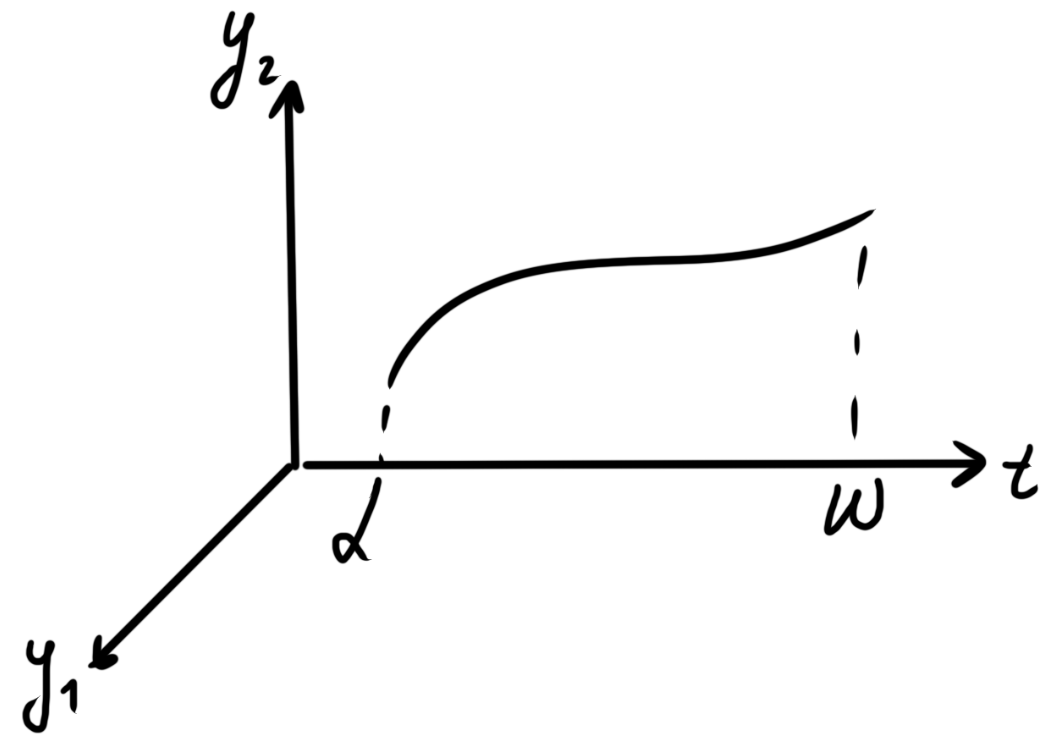
\includegraphics[width=0.6\textwidth]{/Users/vladbelousov/Desktop/Semestr_4-FP-NSU/ДфУ/Лекции_по_дням/image/65.png}
\end{center}

\textbf{Интегральная кривая} - график функции \( \vec{y } (t )  \), то есть множество точек \( \{(t, y_1(t ), ..., y_n (t ) ) , t \in (\alpha , \omega )\} \) \\

\textbf{Фазовое пространство} - пространство переменных \( \{y_1, \ldots,y_n\} \) 

\begin{center}
    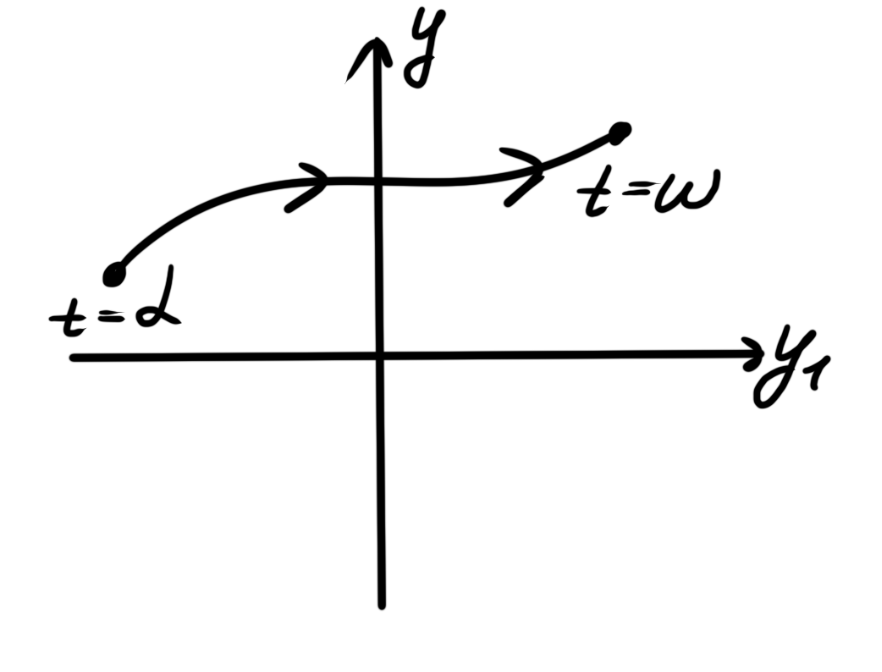
\includegraphics[width=0.4\textwidth]{/Users/vladbelousov/Desktop/Semestr_4-FP-NSU/ДфУ/Лекции_по_дням/image/66.png}
\end{center}

\textbf{Фазовая траектория} - проекция интегральной кривой на фазовое пространство.\\ 

\textbf{Фазовый портрет}  - совокупность фазовых траекторий.

\begin{theorem}
    Для автономных систем фазовые траектории либо не пересекаются, либо совпадают.
\end{theorem}

\begin{proof} \(  \) 

    Пусть \( \begin{aligned}
        \vec{y } (t ) , t \in  (\alpha , \omega ) \\ 
        \vec{ z }  (t ) , t \in  (\alpha , \omega ) 
    \end{aligned}  \) - непродолжаемые  решения системы (1) 

    \[ \begin{aligned}
    \{(y_1 (t ) , ...,y_n(t )), t \in (\alpha_1 , \omega_1 )     \} \\
    \{(z_1 (t ) , ...,z_n (t )), t \in (\alpha_2 , \omega_2 )\}
    \end{aligned}\text{ - траектории системы (1)}  \] 

    \begin{center}
        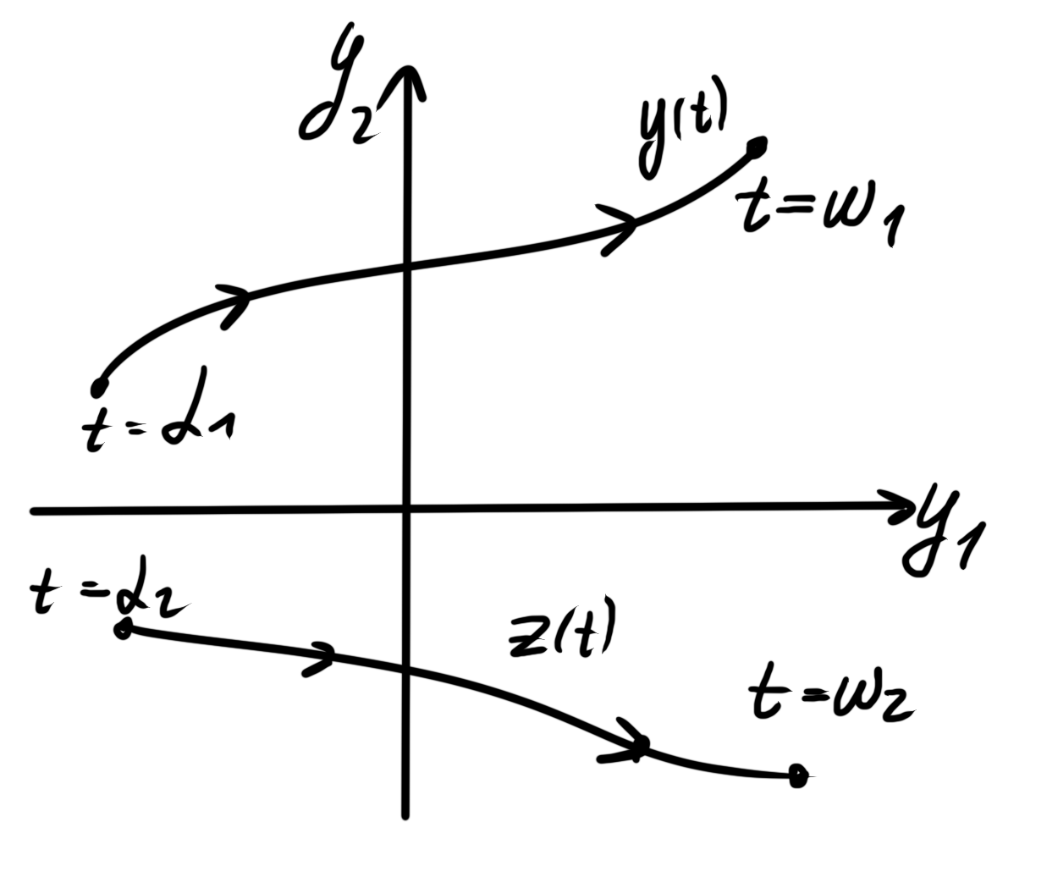
\includegraphics[width=0.5\textwidth]{/Users/vladbelousov/Desktop/Semestr_4-FP-NSU/ДфУ/Лекции_по_дням/image/67.png}
    \end{center}

    Траектории либо пересекаются, либо нет. Если он не пересекаются, то все доказано. Пусть траектории пересекаются: 

    \begin{center}
        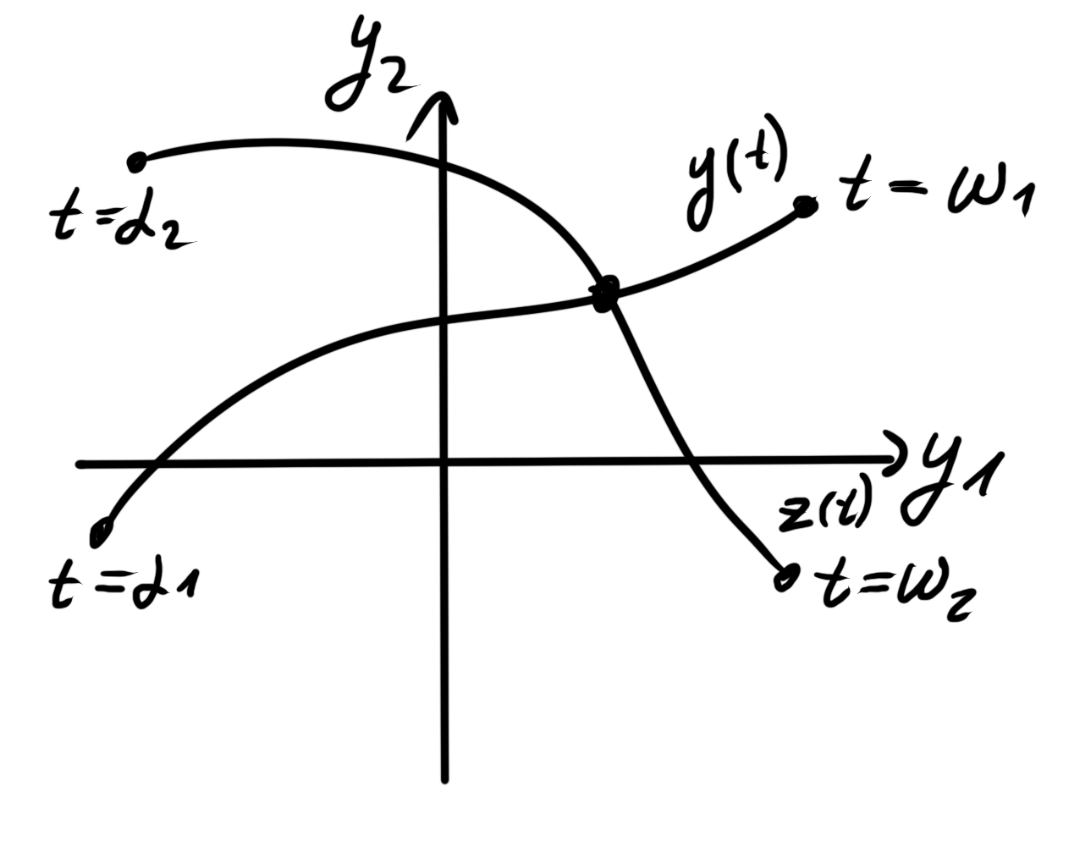
\includegraphics[width=0.5\textwidth]{/Users/vladbelousov/Desktop/Semestr_4-FP-NSU/ДфУ/Лекции_по_дням/image/68.png}
    \end{center}

    \( \Rightarrow \exists  t_1 \in  (\alpha_1 , \omega_1 ) \text{ }  \exists  t_2 \in (\alpha_2 , \omega_2 ) : \vec{y} (t_1 )= \vec{z }  (t_2) \) \\

    \(  \Rightarrow \) по Теореме 1 \( \exists c : \vec{ z } (t ) = \vec{ y} (t + c ) , \text{ }  (\alpha_2 , \omega_2 ) = (\alpha_1  - c , \omega_1 - c ) , \text{ }  c = t_1 -t_2 \) 

    Покажем, что траектории совпадают: 
    \[ \{(z_1(t) , ..., z_n(t )) , t \in  (\alpha_2 , \omega_2 )   \} = \{(y_1 (t +c ) ,..., y_n(t +c )), \underbrace{t \in  (\alpha_1 - c , \omega_1 - c )}_{t +c \in  (\alpha_1 , \omega_1)}\} \] 
    , сделаем замену \( s = t +c  \): 

    \[ \{(y_1 (t +c ) ,..., y_n(t +c )), t \in  (\alpha_1 - c , \omega_1 - c )\}=\{(y_1(s ), ...,y_n(s )) s \in (\alpha_1 , \omega_1)\} \] 
    
\end{proof}

\begin{theorem} 
    Для автономных систем существует 3 типа фазовых траекторий: 

    1) точка; 

    2) замкнутая крива (цикл); 

    3) кривая без самопересечений.

\end{theorem}

\begin{proof} \(  \) 

    Пусть \( \vec{y } (t ) , t \in (\alpha , \omega ) \) - непродолжаемое решение системы (1) \\

    1) \( \forall  t_1 \neq  t_2 : \vec{ y} (t_1 ) \neq  \vec{ y} (t_2 ) \) 

    \begin{center}
        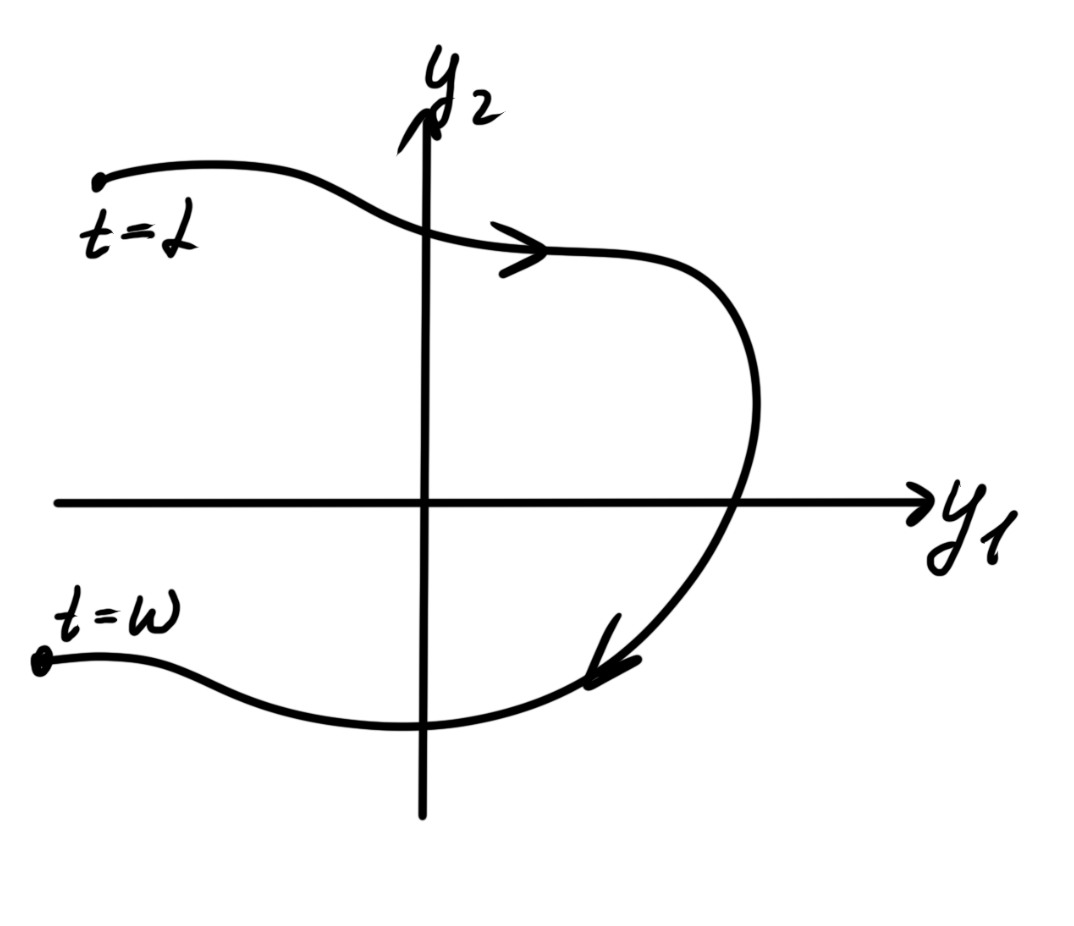
\includegraphics[width=0.4\textwidth]{/Users/vladbelousov/Desktop/Semestr_4-FP-NSU/ДфУ/Лекции_по_дням/image/69.png}
    \end{center}
    - кривая без самопересечений. \\

    2) \( \exists  t_1 \neq  t_2 : \vec{ y } (t_1 ) = \vec{ y } (t_2 ) - \vec{ y}_0 \) 

    \kern+1cm 2a) \( \forall  t  \in  (\alpha , \omega ) : \vec{ y }  (t ) = \vec{ y} _0 \) 

    \begin{center}
        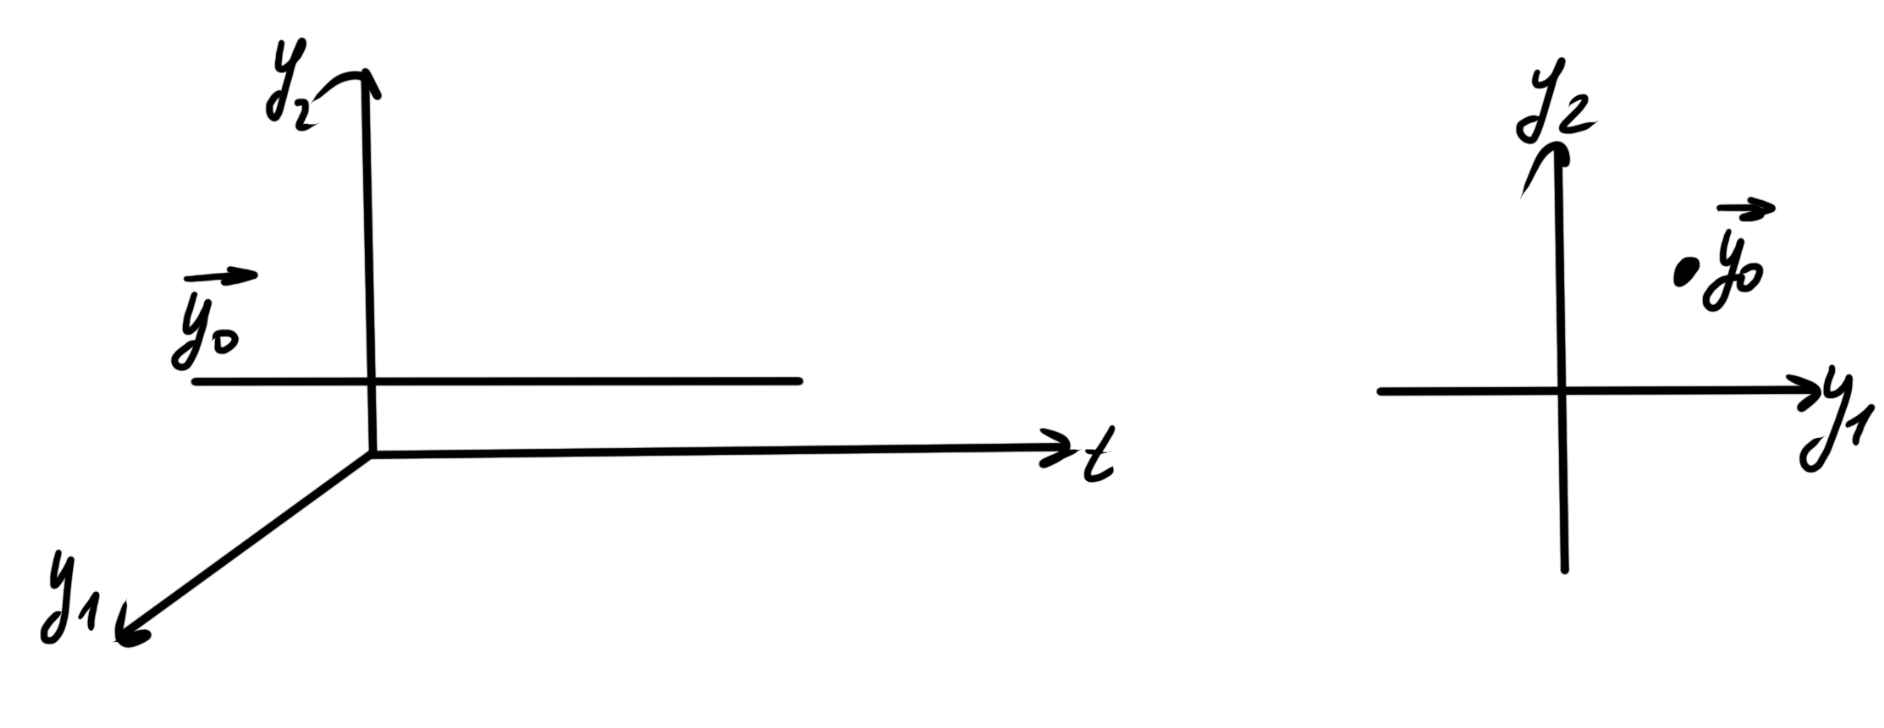
\includegraphics[width=0.8\textwidth]{/Users/vladbelousov/Desktop/Semestr_4-FP-NSU/ДфУ/Лекции_по_дням/image/70.png}
    \end{center}

    \kern+1cm 2б) \( \exists  t_3 \neq  t_1 , \text{  } t_3 \neq  t_2 : \vec{ y}  (t_3 ) \neq  \vec{ y} _0 \) 

    По Теореме 1: \( \begin{cases}
    \vec{ y}  (t ) , t \in (\alpha_1 , \omega_1 ) = (\alpha , \omega ) \\
    \vec{y } (t ) , t \in  (\alpha_2 , \omega_2 ) = (\alpha , \omega)
    \end{cases} \), \( \exists  t 1 \in (\alpha  ,\omega ) , \text{ }  \exists t_2 \in  (\alpha, \omega ) : \vec{ y } (t_1 ) =\vec{ y}  (t_2 ) \) \\

    \( \Rightarrow \exists  c \in  \mathbb{R} : \vec{ y}  (t ) = \vec{ y}  (t  + c ), \text{ }  (\alpha , \omega ) = (\alpha -c , \omega - c ), \text{ }  c = t_1 -t_2 \neq  0  \)     

    \begin{center}
        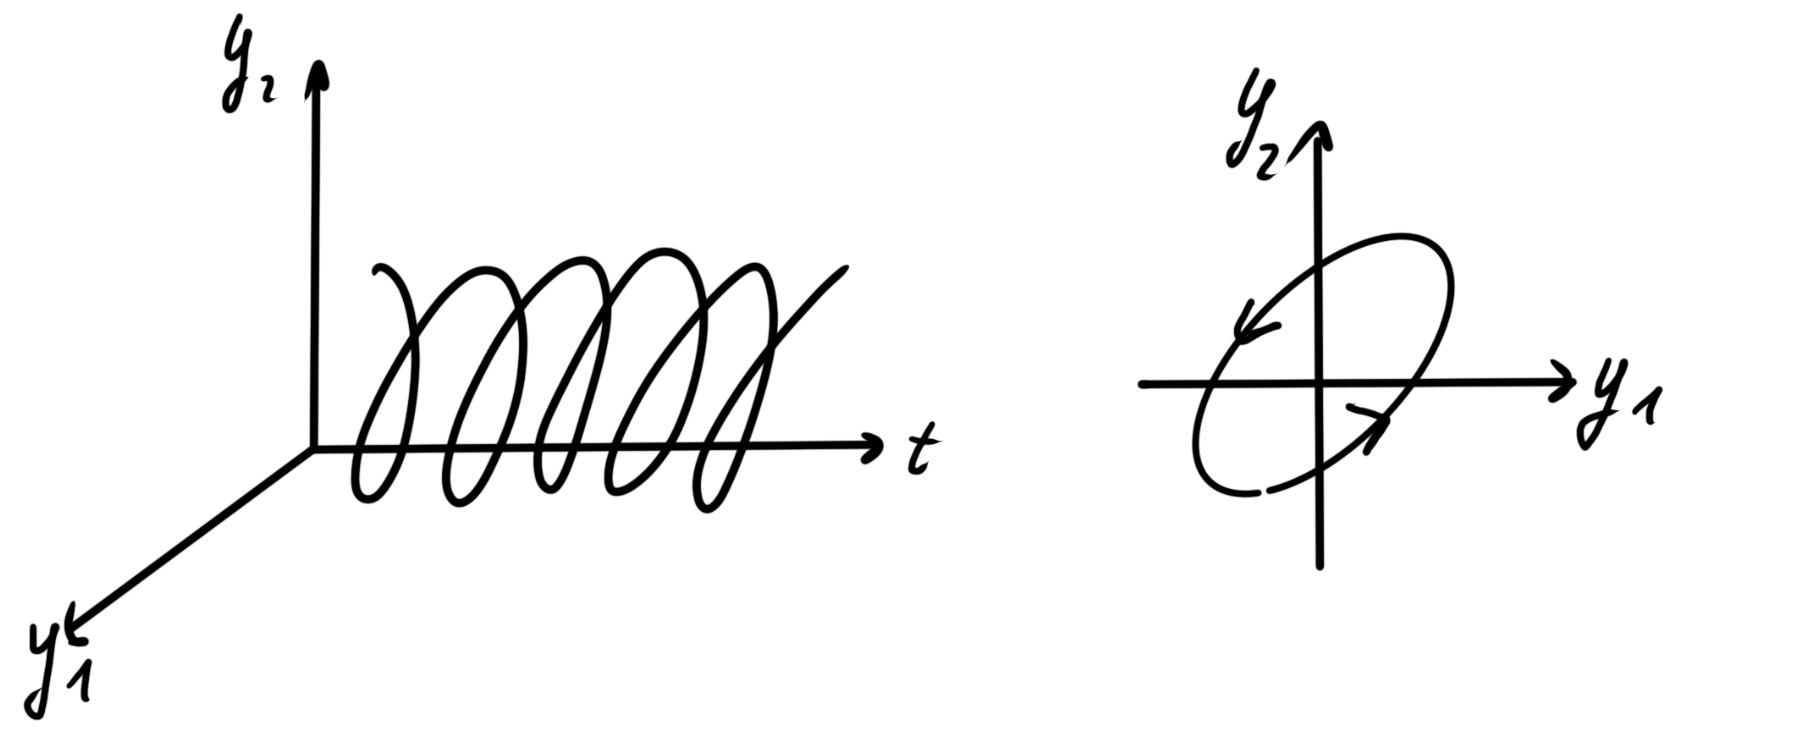
\includegraphics[width=0.5\textwidth]{/Users/vladbelousov/Desktop/Semestr_4-FP-NSU/ДфУ/Лекции_по_дням/image/71.png}
    \end{center}

\end{proof}

\chapter{Уравнения с частными производными}

\section{Первые интегралы систем обыкновенных дифференциальных уравнений}

\[ \frac{d}{dt }  \vec{ y}  = \vec{ f } (t, \vec{ y}  ) \tag{1} \] 
, где \( \vec{y }  = \begin{pmatrix}
y_1 \\
\vdots\\
y_n
\end{pmatrix} , \vec{f } (t, \vec{ y}  ) = \begin{pmatrix}
f_1(t, \vec{y } )\\
\vdots\\
f_n(t, \vec{ y} )
\end{pmatrix}, \text{ }  f_j : \mathbb{D} \to  \mathbb{R} , \mathbb{D} \subset \mathbb{R}^{n+1} \) 

Выполняется условие Теоремы Пикара: \( f_j \in  C(\mathbb{D} ), \exists  \frac{\partial  f_i }{\partial  y_j } \in  C(\mathbb{D} ) , \text{ }  i,j = 1, \ldots,n  \) 

\begin{definition}
    функция \( \Phi (t, \vec{y } ) = \Phi(t, y_1 , ..., y_n )  \) называется первым интегралом системы (1), если \( \forall  \vec{y} (t ) \) системы (1) выполняется \( \Phi(t, \vec{ y}  (t )) = \mathrm{const}   \) 
\end{definition}

Пример: 

\[ \begin{cases}
x ' = x \\ 
y ' = -y
\end{cases} \quad  \Phi(t, x ,y) = x y \neq  \mathrm{const}   \] 

\[ \begin{cases}
    x(t )  = e^t c_1 \\
    y(t ) = e^{-t }  c_2
\end{cases}\quad  \Phi(t,x(t ), y(t )) = x(t ) y (t ) = c_1 c_2 = \mathrm{const }  \Rightarrow xy \text{ - первый интеграл.}  \]

\textbf{Замечание 1. } 

Если \( \Phi \in  C^1 , \text{ }  \Phi(t ,\vec{ y}  )  \)  - первый интеграл, то \( \displaystyle \frac{d}{dt }  \Phi(t, \vec{ y}  (t ))= 0 \)  \\

Проверим, что \( \Phi = xy  \) - первый интеграл, не зная решения. 

\[ \Phi(t, x(t ), y(t )) = x(t )  y(t ) \] 
\[ \frac{d}{dt }  \Phi(t, x(t ), y(t )) = x' (t )y (t ) + x(t ) y'(t ) =0 \] 

\begin{theorem}
    Пусть \( \Phi(t,\vec{y } ) \in  C^1 (\mathbb{D} )  \). Функция \( \Phi(t, \vec{ y} ) \)  - первый интеграл системы (1) \( \Leftrightarrow    \Phi(t, \vec{ y} )  \) - решение уравнения с частными производными. 

    \[ \frac{\partial  }{\partial  t } \Phi + f_1 (t , \vec{ y} ) \frac{\partial  \Phi }{\partial  y_1 }+ ... + f_n (t , \vec{ y} ) \frac{\partial  \Phi }{\partial  y_n } = 0 \tag{2}    \] 
\end{theorem}

\begin{proof} \(  \) 

    \( (\Rightarrow): \) 

    Пусть \( \Phi(t, \vec{y } )  \) - первый интеграл. Пусть \( (t_0 ,\vec{y} _0 ) \)  - произвольная точка из \( \mathbb{D} \) 

    \[ \begin{cases}
    \displaystyle  \frac{d}{dt }  \vec{ y}  = \vec{f } (t, \vec{y } ) \\ 
    \vec{ y } (t_0 ) = \vec{ y} _0 
    \end{cases} \Rightarrow \vec{y } (t ) \text{ - решение } t \in  (\alpha , \omega) \Rightarrow \Phi(t, \vec{y } (t )) = \mathrm{const }  \Rightarrow \frac{d}{dt }  \Phi(t, \vec{ y} (t )) =0  \] 

    \[ \frac{\partial  \Phi }{\partial  t }(t, \vec{ y}  (t )) + \frac{\partial  \Phi }{\partial  y_1 } (t, \vec{ y}  (t )) \underbrace{\frac{d y_1 (t )}{dt }}_{f_1(t,\vec{ y} (t))} +... + \frac{\partial  \Phi }{\partial y_n }(t , \vec{ y}  (t )) \underbrace{ \frac{d y_n (t )}{dt }}_{f_n(t, \vec{ y} (t))} = 0   , \text{ }  \forall  t \in  (\alpha , \omega )   \] 

    \[ t =t_0 : \frac{\partial  \Phi }{\partial  t } (t_0 ,\vec{ y}_0 ) + \frac{\partial  \Phi }{\partial  y_1 } (t_0 ,\vec{ y} _0 )f_1 (t_0, \vec{ y} _0 )+... + \frac{\partial  \Phi }{\partial  y_1 }(t_0 , \vec{ y} _0) f_n (t_0 ,\vec{ y} _0 ) = 0 , \text{ }  \forall  (t_0 , \vec{ y} _0 )\in  \mathbb{D}     \] \\

    \( (\Leftarrow): \) 

    Пусть \( \Phi(t, \vec{ y} ) \) - решение уравнения (2): 

    \[ \frac{\partial  }{\partial  } \Phi(t, \vec{ y}  ) + f_1 (t, \vec{ y}  ) \frac{\partial  \Phi }{\partial  y_1 } (t ,\vec{ y}  )+ ... + f_n (t, \vec{ y} ) \frac{\partial \Phi }{\partial  y_n }(t, \vec{ y}  ) =0 , \text{ }  \forall  (t, \vec{ y} ) \in \mathbb{D}   \] 

    Возьмем \( \vec{ y } = \vec{ y } (t ) \) - решение системы (2) 

    \[ \frac{\partial  }{\partial  t } \Phi(t, \vec{ y} (t )) + \sum_{j =1}^{n }   \underbrace{ f_j (t,\vec{ y} (t )) }_{\frac{d}{dt } y_j(t)}\frac{\partial  \Phi }{\partial  y_j }(t, \vec{ y} (t ) ) = \frac{d}{dt }  \Phi(t,\vec{ y} (t )) \Rightarrow \Phi(t, \vec{ y} (t )) = \mathrm{const}     \] 

\end{proof}

Пример: 

\[ \begin{cases}
x ' = x \\ 
y ' = - y 
\end{cases} \quad  \begin{aligned}
    \Phi_1 (t,x,y ) &= xy  \quad  \Phi_3 = 3xy + 4 \quad  \Phi_5 = \displaystyle \frac{1}{xy }  \\ 
    \Phi_2 &= 2 xy \quad  \Phi_4=  (xy )^2 \quad  \Phi_6 = F(xy)
\end{aligned}\] 

\begin{theorem}
    Пусть \( \Phi_1 (t, \vec{ y}  ), ..., \Phi_k(t, \vec{ y} ) \) - первые интегралы системы (1), \( F(z_1, \ldots, z_k) \) - произвольная функция. Тогда \( F(\Phi_1 (t,\vec{ y} ), ..., \Phi_k (t , \vec{y} )) \) - тоже первый интеграл системы (1).
\end{theorem}

\begin{proof} \(  \) 

    По Определению \(  \Phi_j (t,\vec{ y} (t )) = c_j = \mathrm{const}  , \text{ }  j = 1, \ldots, k , \text{ }  \vec{ y } (t )\) - решение (1)

    \[ F(\underbrace{ \Phi_1 (t, \vec{ y} (t ))}_{c_1}, ..., \underbrace{\Phi_k (t, \vec{ y} (t ))}_{c_k}) = F(c_1, \ldots, c_k ) = \mathrm{const } \Rightarrow F(\Phi_1 ,..., \Phi_k) \text{ - первый интеграл}  \] 

\end{proof}

\begin{definition}
    Пусть \( \Phi_1(t, \vec{ y} ) ,... , \Phi_k (t, \vec{y } ) \in  C^1 (\mathbb{D}) \). Функции \( \Phi_1 ,..., \Phi_k  \) называются функционально независимыми в области \( \mathbb{D} \) если: 

    \[ \rank \begin{pmatrix}
    \displaystyle \frac{\partial \Phi_1 }{\partial  t }  & \displaystyle \frac{\partial  \Phi_1 }{\partial  y_1 }  & \dots & \displaystyle  \frac{\partial  \Phi_1 }{\partial y_n} \\[10pt]
    \dots & \dots& \dots &\dots \\[10pt]
    \displaystyle \frac{\partial  \Phi_k}{\partial t}  & \displaystyle  \frac{\partial  \Phi_k }{\partial y_1}  & \dots & \displaystyle  \frac{\partial  \Phi_k }{\partial  y_n} 
    \end{pmatrix} _{k \times  (n+1)}  =k  ,\text{ }  \forall  (t, \vec{ y}  )\in  \mathbb{D} \] 
\end{definition}

\textbf{Замечание 1.} 

Если \( \Phi_1 ,...,\Phi_k  \) функционально независимы, то они друг через друга не выражаются. 

От противного: пусть \(  \Phi_1 = F(\Phi_2 , ..., \Phi_k) \quad  \Phi_1 (t, \vec{ y} ) = F(\Phi_2 (t,\vec{ y} ),..., \Phi_k (t, \vec{ y} ))\) 

\[ \begin{cases}
\displaystyle  \frac{\partial  \Phi_1 }{\partial  t } = \frac{\partial F }{\partial  \Phi_2 } \frac{\partial  \Phi_2 }{\partial t    } +...+ \frac{\partial  F }{\partial  \Phi_k }    \frac{\partial  \Phi_k }{\partial  t} \\[10pt] 
\displaystyle  \frac{\partial  \Phi_1 }{\partial  y_1} = \frac{\partial F }{\partial  \Phi_2 } \frac{\partial  \Phi_2 }{\partial y_1   } +...+ \frac{\partial  F }{\partial  \Phi_k }    \frac{\partial  \Phi_k }{\partial  y_1}  \\
\vdots \\ 
\displaystyle  \frac{\partial  \Phi_1 }{\partial  y_n } = \frac{\partial F }{\partial  \Phi_2 } \frac{\partial  \Phi_2 }{\partial y_n    } +...+ \frac{\partial  F }{\partial  \Phi_k }    \frac{\partial  \Phi_k }{\partial  y_n} 
\end{cases} \] 

\[ \underbrace{\begin{pmatrix}
    \displaystyle \frac{\partial  \Phi_1 }{\partial  t }\\[10pt]
    \displaystyle \frac{\partial  \Phi_1 }{\partial  y_1 }\\
\vdots\\
\displaystyle \frac{\partial  \Phi_1 }{\partial  y_n }
\end{pmatrix}}_{\text{1-ая строка} } = \frac{\partial  F }{\partial  \Phi_2} \underbrace{\begin{pmatrix}
    \displaystyle \frac{\partial  \Phi_2 }{\partial t    } \\[10pt]
\displaystyle  \frac{\partial  \Phi_2 }{\partial y_1    } \\
\vdots\\
\displaystyle  \frac{\partial  \Phi_2 }{\partial y_n   } 
\end{pmatrix}}_{\text{2-ая строка} } +... + \frac{\partial  F }{\partial  \Phi_k } \underbrace{\begin{pmatrix}
    \displaystyle   \frac{\partial  \Phi_k }{\partial  t}  \\[10pt]
    \displaystyle   \frac{\partial  \Phi_k }{\partial  y_1} \\
    \vdots\\
    \displaystyle  \frac{\partial  \Phi_k }{\partial  y_n} 
    \end{pmatrix}}_{\text{k-ая строка} }  \Rightarrow \rank (... )< k \]
    
    \textbf{Замечание 2.}
    
    Пусть в Определении 2 \( \Phi_1, ...,\Phi_k \) - первые интегралы. Тогда в матрице из Определения 2 можно не учитывать первый столбец (следует из Теоремы 1)

    



%%-------------------------------%%

% Закрытие документа, если файл компилируется отдельно
\ifdefined\mainfile
    % Если это основной файл, не нужно заканчивать документ
\else
    \end{document}
\fi